\subsection{Resources}

\begin{frame}
  \frametitle{Applications Resources}
  \begin{itemize}
  \item Applications contain more than just compiled source code:
    images, videos, sound, etc.
  \item In Android, anything related to the visual appearance of the
    application is kept separate from the source code: activities
    layout, animations, menus, strings, etc.
  \item Resources should be kept in the \code{res/} directory of your
    application.
  \item At compilation, the build tool will create a class \code{R},
    containing references to all the available resources, and
    associating an ID to it
  \item This mechanism allows you to provide several alternatives to
    resources, depending on locales, screen size, pixel density,
    etc. in the same application, resolved at runtime.
  \end{itemize}
\end{frame}

\begin{frame}
  \frametitle{Resources Directory}
  \begin{itemize}
  \item All resources are located in the \code{res/} subdirectory
    \begin{itemize}
    \item \code{anim/} contains animation definitions
    \item \code{color/} contains the color definitions
    \item \code{drawable/} contains images, "9-patch" graphics, or XML-files
      defining drawables (shapes, widgets, relying on a image file)
    \item \code{layout/} contains XML defining applications layout
    \item \code{menu/} contains XML files for the menu layouts
    \item \code{raw/} contains files that are left untouched
    \item \code{values/} contains strings, integers, arrays,
      dimensions, etc
    \item \code{xml/} contains arbitrary XML files
    \end{itemize}
  \item All these files are accessed by applications through their
    IDs. If you still want to use a file path, you need to use the
    \code{assets/} folders
  \end{itemize}
\end{frame}

\begin{frame}
  \frametitle{Resources}
  \begin{figure}[h!]
    \centering
    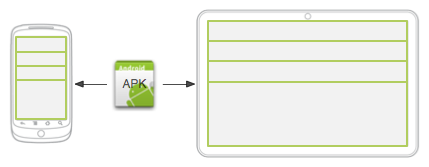
\includegraphics[height=0.4\textheight]{slides/android-application-resources/resource-no-alternative.png}\\
    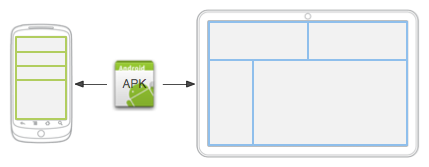
\includegraphics[height=0.4\textheight]{slides/android-application-resources/resource-alternative.png}\\
    {
      \tiny
      Credits: \url{http://developer.android.com}
    }
  \end{figure}
\end{frame}

\begin{frame}
  \frametitle{Alternative Resources}
  \begin{itemize}
  \item Alternative resources are provided using extended sub-folder
    names, that should be named using the pattern
    \code{<folder_name>-<qualifier>}
  \item There is a number of qualifiers, depending on which case
    you want to provide an alternative for. The most used ones are probably:
    \begin{itemize}
    \item locales (\code{en}, \code{fr}, \code{fr-rCA}, ...)
    \item screen orientation (\code{land}, \code{port})
    \item screen size (\code{small}, \code{large},...)
    \item screen density (\code{mdpi}, \code{ldpi}, ...)
    \item and much others
    \end{itemize}
  \item You can specify multiple qualifiers by chaining them,
    separated by dashes. If you want layouts to be applied only when
    on landscape on high density screens, you will save them into the
    directory \code{layout-land-hdpi}
  \end{itemize}
\end{frame}

\begin{frame}
  \frametitle{Resources Selection}
  \begin{figure}[h!]
    \centering
    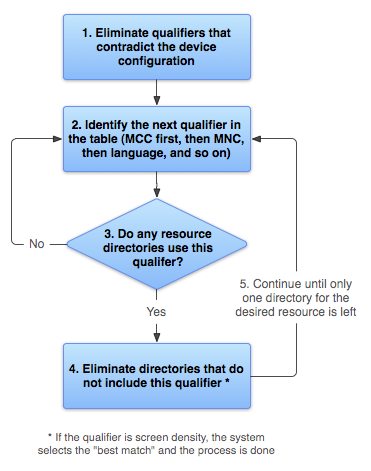
\includegraphics[height=0.8\textheight]{slides/android-application-resources/resource-selection.png}\\
    {
      \tiny
      Credits: \url{http://developer.android.com}
    }
  \end{figure}
\end{frame}
